\section{Arquitetura e Implementação do Protótipo}
\label{referencial}

\subsection{Escopo e Arquitetura}

Nesta etapa foi desenvolvido um protótipo utilizando o middleware NATS, com o objetivo de demonstrar a comunicação distribuída entre processos executando em máquinas físicas distintas. O protótipo segue o paradigma de mensageria \textit{publish/subscribe}, permitindo que um cliente envie solicitações e receba respostas processadas por um servidor.


A comunicação entre cliente e servidor ocorre por meio de subjects do NATS, garantindo desacoplamento entre os processos e permitindo escalabilidade para múltiplos clientes ou múltiplos serviços.

\begin{figure}[ht]
\centering
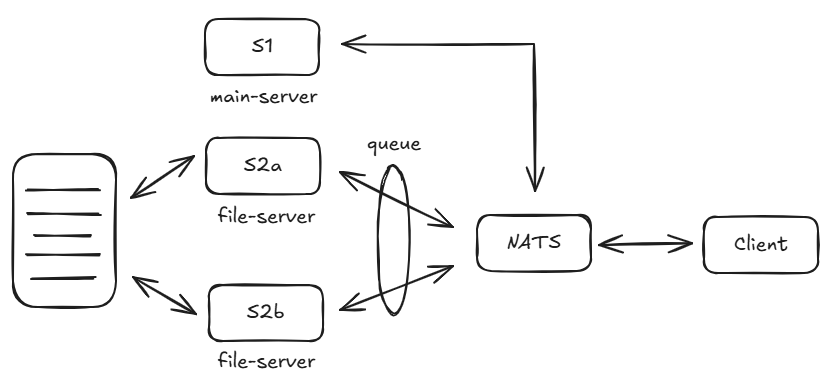
\includegraphics[width=1.0\linewidth]{figs/diagrama_arquitetura.png}
\caption{Diagrama da Arquitetura do Protótipo.}
\label{fig:diagrama_arquitetura}
\end{figure}



\subsection{Operações Implementadas}

\begin{enumerate}
    \item \textbf{Resposta a mensagem de texto}: O cliente publica uma requisição textual em um subject dedicado, que é consumida pelo serviço principal S1. O S1 realiza o parsing da mensagem, processa o conteúdo e retorna uma resposta ao cliente utilizando o padrão request/reply do NATS, validando a troca de mensagens com baixa latência.

    \item \textbf{Alteração de arquivo no servidor}: O cliente envia uma requisição contendo os dados a serem persistidos diretamente ao serviço de arquivos por meio de um subject específico. O processamento é realizado por uma das instâncias S2a ou S2b, configuradas em queue group, garantindo balanceamento de carga entre os servidores. A instância selecionada executa a escrita/atualização do arquivo local e retorna ao cliente o status da operação utilizando o mecanismo de request/reply do NATS.

    \item \textbf{Cálculo de Funções}: O cliente solicita a execução de uma função matemática enviando parâmetros e o tipo de operação desejada. O serviço S1 interpreta a requisição, executa o cálculo e retorna o resultado ao cliente via NATS, utilizando request/reply. Essa operação evidencia o uso do middleware para processamento remoto orientado a mensagens.
    
\end{enumerate}

\subsection{Configuração do Ambiente}

Para a execução do protótipo, foi necessária a configuração do servidor NATS e das dependências da linguagem escolhida.

Inicialmente, o servidor NATS foi executado na máquina responsável pelo broker utilizando o comando: nats-server.

Em seguida, cliente e servidor foram executados em máquinas físicas distintas, conectadas à mesma rede, configurando o endereço IP do servidor NATS para permitir comunicação remota.

Além disso, foi utilizada a biblioteca oficial do NATS para a linguagem escolhida, responsável por estabelecer conexão, publicar mensagens e realizar subscriptions nos subjects definidos.

\section{Evidências Técnicas}

\subsection{Fluxo de Comunicação}

O fluxo de comunicação do protótipo ocorre de forma indireta e desacoplada, sendo mediado pelo middleware NATS, que atua como broker central responsável pelo roteamento das mensagens. O cliente envia requisições publicando mensagens em subjects específicos, e o NATS encaminha essas mensagens aos serviços inscritos nos respectivos canais.

Para operações de texto e cálculo, as mensagens são encaminhadas diretamente ao serviço principal S1 (main-server), que processa a solicitação e retorna uma resposta ao cliente utilizando o mecanismo de request/reply do NATS. Dessa forma, o cliente recebe a resposta sem necessidade de conexão direta com o servidor.

Para operações envolvendo manipulação de arquivos, o cliente publica a requisição diretamente no subject correspondente ao serviço de arquivos. Essa requisição é entregue a apenas uma das instâncias do serviço (S2a ou S2b) devido ao uso de queue group, permitindo balanceamento de carga entre servidores e evitando processamento duplicado. A instância selecionada realiza a operação no armazenamento e retorna o resultado ao cliente por meio do mecanismo de request/reply do NATS. Esse modelo promove maior desacoplamento entre os componentes, além de permitir escalabilidade horizontal e maior tolerância a falhas no serviço de arquivos.

\subsection{Resultados}

Os testes realizados demonstraram que o protótipo implementado com NATS foi capaz de executar corretamente as operações propostas, garantindo comunicação distribuída eficiente entre os componentes. Em todas as requisições enviadas pelo cliente, o sistema retornou respostas estruturadas em formato JSON, contendo código de status, mensagem descritiva e os dados correspondentes ao processamento.


\begin{figure}[ht]
\centering
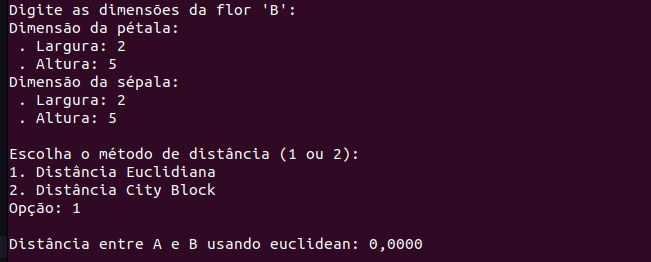
\includegraphics[width=0.75\linewidth]{figs/client-1.png}
\caption{Cálculo de funções.}
\label{fig:resultado}
\end{figure}

\begin{figure}[ht]
\centering
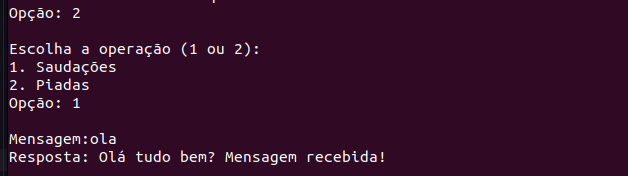
\includegraphics[width=0.75\linewidth]{figs/client-2.png}
\caption{Resposta a mensagem de texto.}
\label{fig:resultado}
\end{figure}

\begin{figure}[ht]
\centering
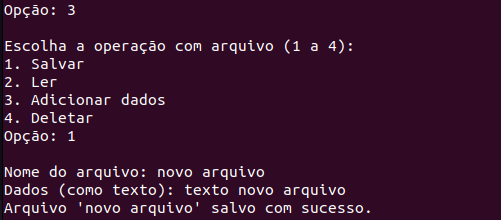
\includegraphics[width=0.75\linewidth]{figs/client-3.png}
\caption{Alteração de arquivo.}
\label{fig:resultado}
\end{figure}


\begin{figure}[ht]
\centering
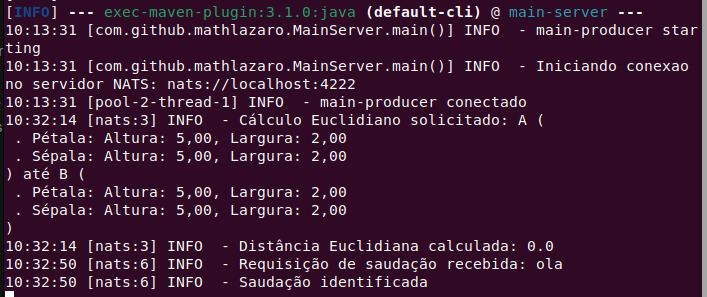
\includegraphics[width=0.75\linewidth]{figs/servidor-mensagem.jpeg}
\caption{Servidor resposta a mensagem.}
\label{fig:resultado}
\end{figure}


\begin{figure}[ht]
\centering
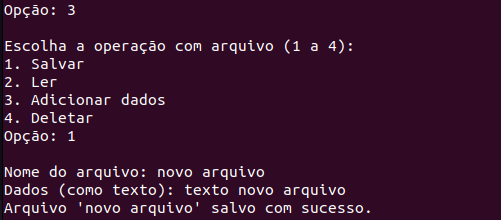
\includegraphics[width=0.75\linewidth]{figs/client-3.png}
\caption{Servidor alteração de arquivo.}
\label{fig:resultado}
\end{figure}


Conforme evidenciado na execução, a operação de envio de mensagem, alteração de arquivo ou cálculo matemático foi concluída com sucesso, retornando mensagens de confirmação como "Operação realizada com sucesso" e status 200, indicando que o fluxo de comunicação baseado em request/reply funcionou corretamente. Dessa forma, os resultados validam que o NATS realizou o roteamento das mensagens de forma adequada e que os serviços distribuídos foram capazes de processar e responder às solicitações conforme o esperado.

\label{ssec:alg}